% --- LLM inference: prefill vs.\ decode ---
% ========== Part 1: Inference optimisation ==========
\begin{frame}{Understanding LLM Inference}
  \begin{columns}[T,onlytextwidth]
    \column{0.52\textwidth}
      \begin{itemize}\footnotesize
        \item[\textcolor{red}{$\blacktriangleright$}] Most popular decoder-only LLMs (e.g., GPT-3) are pretrained for \textbf{causal language modeling}: predicting the next token in a sequence.
        \item[\textcolor{red}{$\blacktriangleright$}] At inference, LLMs receive a series of \textbf{tokens} as input and generate the following tokens \textbf{autoregressively} until a stopping criterion is met\\
          {\scriptsize (e.g., token limit, stop word, or special \texttt{<end>} token).}
        \item[\textcolor{red}{$\blacktriangleright$}] \textbf{Tokens} are about 4 English characters each.
        \item[\textcolor{red}{$\blacktriangleright$}] The inference process has \textbf{two phases}: \textbf{prefill} (process prompt in parallel) and \textbf{decode} (step-by-step token generation).
      \end{itemize}
    \column{0.46\textwidth}
      \centering
      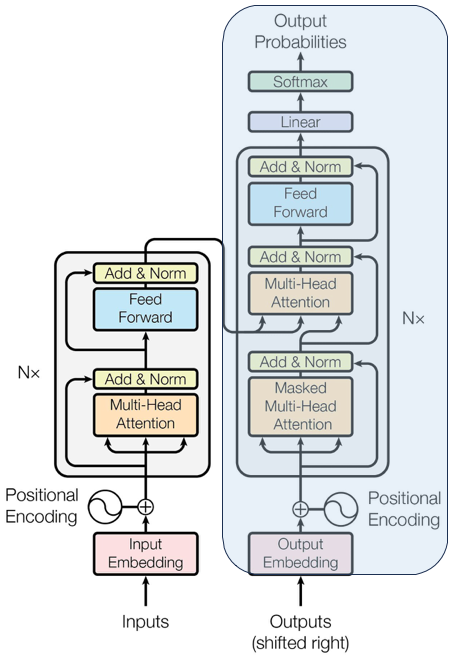
\includegraphics[width=\linewidth,height=0.82\textheight,keepaspectratio]{assets/Lecture-6_Introduction_to_Transformers/pdf_page_094.png}
  \end{columns}
\end{frame}

\begin{frame}{Prefill Phase: Parallel Input Processing}
  \begin{columns}[T,onlytextwidth]
    \column{0.54\textwidth}
      \begin{itemize}\itemsep0.6em
        \item[\textcolor{red}{$\blacktriangleright$}] \textbf{Prefill phase (input processing):}
          \begin{itemize}\itemsep0.25em
            \item All input tokens are processed together to compute \textbf{keys and values} (attention states) for the prompt.
            \item The entire input sequence is known in advance, enabling a highly parallel \textbf{matrix-matrix} computation that fully leverages the GPU's throughput.
          \end{itemize}
        \item[\textcolor{red}{$\blacktriangleright$}] \textbf{Token throughput caveat:}
          \begin{itemize}\itemsep0.25em
            \item Different LLMs may use different \textbf{tokenizers}---so "tokens per second" is not always comparable across models, as token-to-character mappings vary.
          \end{itemize}
      \end{itemize}
    \column{0.44\textwidth}
      \centering
      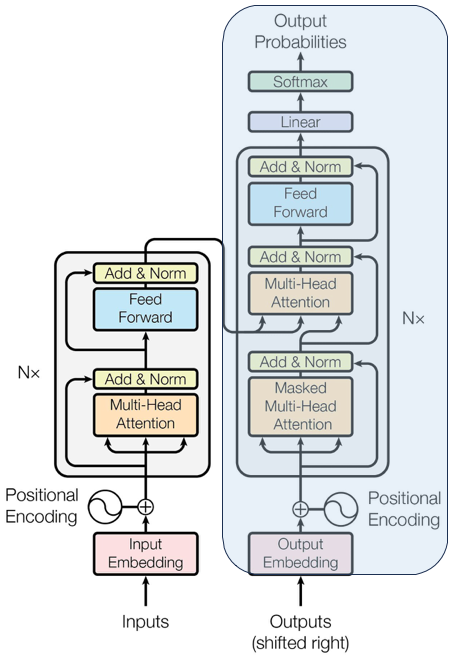
\includegraphics[width=\linewidth,height=0.8\paperheight,keepaspectratio]{assets/Lecture-6_Introduction_to_Transformers/pdf_page_094.png}
  \end{columns}
\end{frame}

\begin{frame}{Decode Phase: Serial Token Generation}
  \begin{columns}[T,onlytextwidth]
    \column{0.55\textwidth}
      \begin{itemize}\itemsep0.6em
        \item[\textcolor{red}{$\blacktriangleright$}] \textbf{Decode phase (generating outputs):}
          \begin{itemize}\itemsep0.25em
            \item Output tokens are generated \textbf{one at a time}, each conditioned on all previously generated tokens.
            \item Computation now becomes a \textbf{matrix-vector} operation---less parallelizable, and typically \textbf{memory-bound}: moving weights/activations dominates speed, not raw compute.
            \item Optimising decode is crucial: efficient attention, key/value caching, and memory management are ongoing research topics.
          \end{itemize}
      \end{itemize}
    \column{0.45\textwidth}
      \centering
      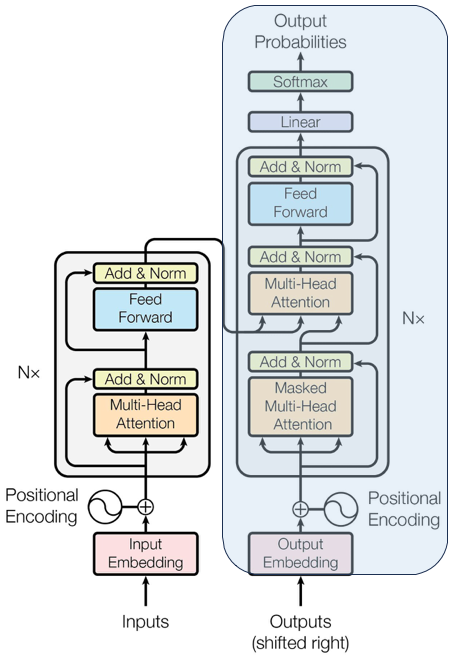
\includegraphics[width=0.9\linewidth,height=0.75\paperheight,keepaspectratio]{assets/Lecture-6_Introduction_to_Transformers/pdf_page_094.png}
  \end{columns}
\end{frame}


\begin{frame}{Why Optimise Inference?}
  \begin{itemize}
    \item[\textcolor{red}{$\blacktriangleright$}] \textbf{Training} is often one-off; \textbf{inference} is repeated at scale (cost, latency, energy).
    \item[\textcolor{red}{$\blacktriangleright$}] Large language models are \textbf{memory-bound} and \textbf{autoregressive}: each new token revisits all previous tokens.
    \item[\textcolor{red}{$\blacktriangleright$}] Goals: lower \textbf{latency} (interactive UX), higher \textbf{throughput} (serving many users), smaller \textbf{memory} (long contexts, edge).
  \end{itemize}
\end{frame}

% \begin{frame}{Transformer Inference: Prefill vs.\ Decode}
%   \begin{columns}[T,onlytextwidth]
%     \column{0.52\textwidth}
%     \begin{itemize}\itemsep0.35em
%       \item[\textcolor{red}{$\blacktriangleright$}] \textbf{Prefill:} process the prompt in parallel (one forward pass over context length).
%       \item[\textcolor{red}{$\blacktriangleright$}] \textbf{Decode:} generate one token at a time; each step attends over \emph{all} past keys and values.
%       \item[\textcolor{red}{$\blacktriangleright$}] Decode dominates cost for long outputs; attention complexity grows with sequence length.
%     \end{itemize}
%     \column{0.46\textwidth}
%     \centering
%     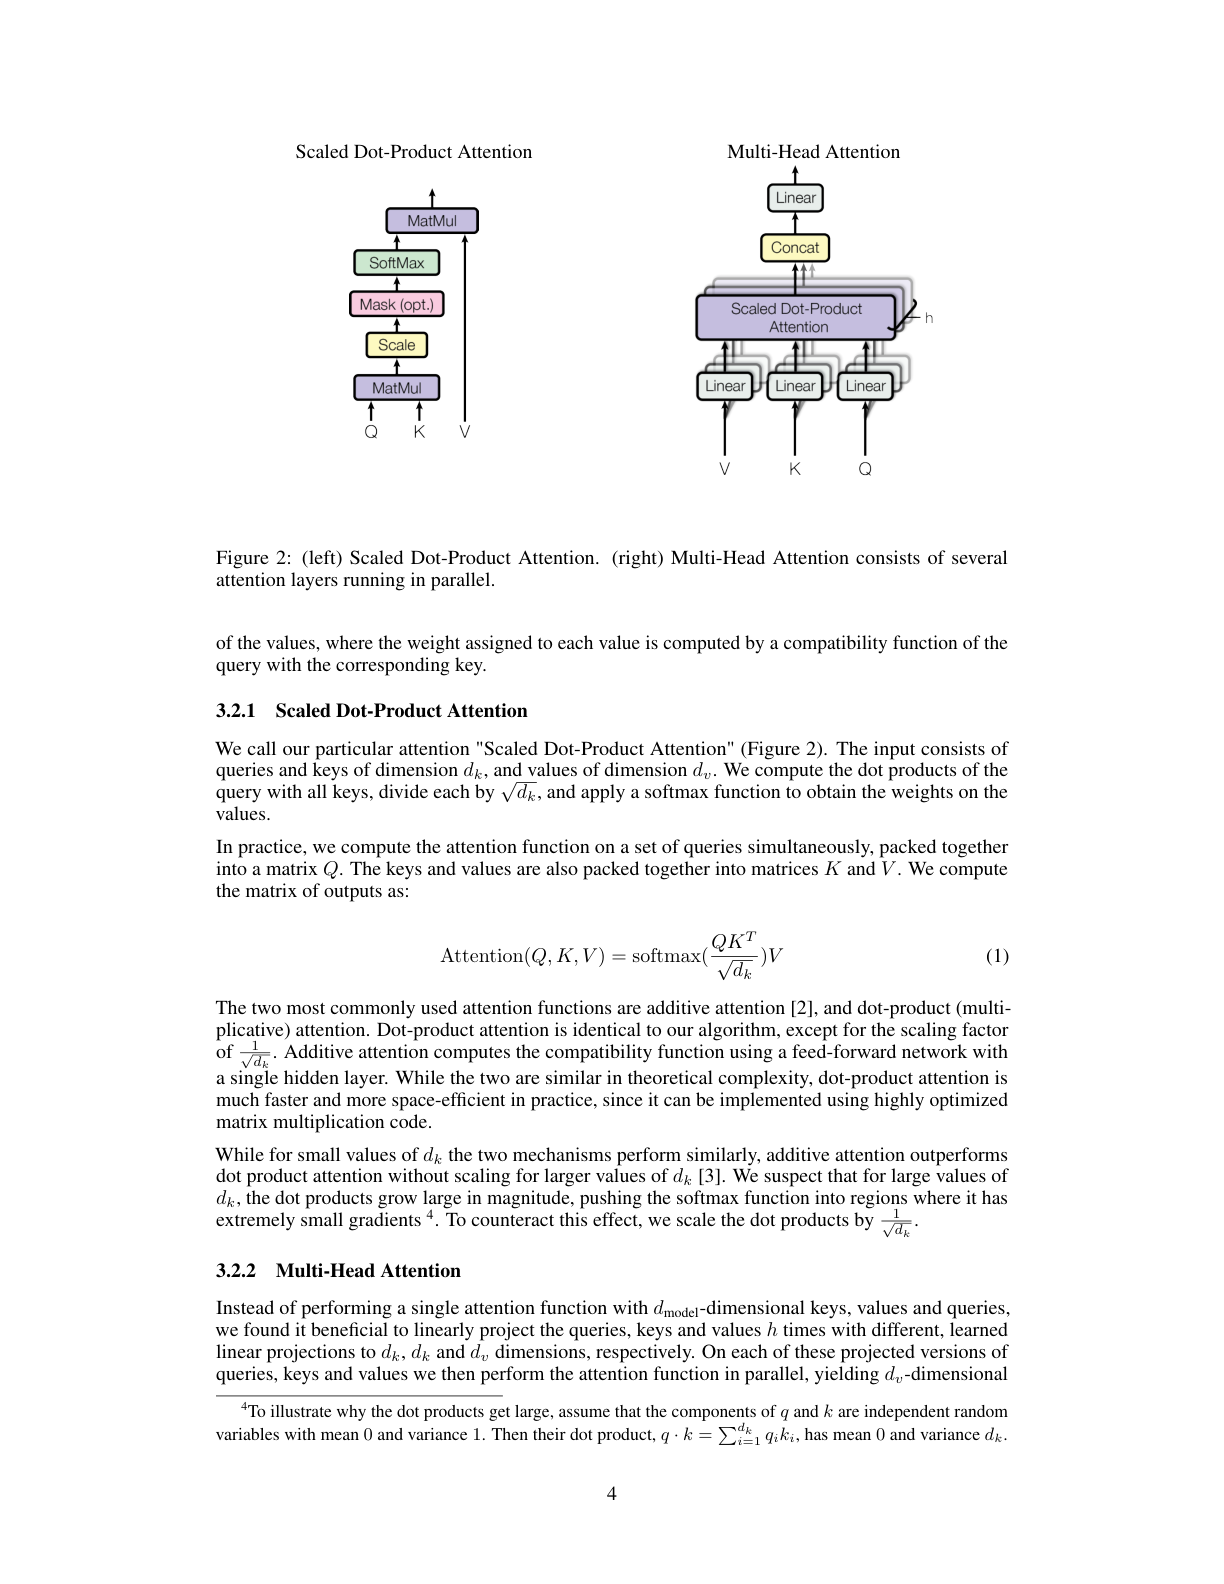
\includegraphics[width=\linewidth,height=0.82\textheight,keepaspectratio]{assets/New-Lecture-Inference_Optimisation/transformer_vaswani_p4.png}\\[-0.2em]
%     {\scriptsize Transformer block (Vaswani et al., 2017).}
%   \end{columns}
% \end{frame}

% \begin{frame}{Inference Optimisation: Key-Value Caching}
%   \begin{columns}[T,onlytextwidth]
%     \column{0.48\textwidth}
%     \begin{itemize}\itemsep0.35em
%       \item[\textcolor{red}{$\blacktriangleright$}] For each layer, cache \textbf{key} and \textbf{value} projections for past tokens.
%       \item[\textcolor{red}{$\blacktriangleright$}] Reuse them at decode time instead of recomputing from hidden states.
%       \item[\textcolor{red}{$\blacktriangleright$}] \textbf{Cost:} memory $\propto$ layers $\times$ heads $\times$ head dim $\times$ sequence length $\times$ batch.
%       \item[\textcolor{red}{$\blacktriangleright$}] Motivates \textbf{quantized KV} (e.g.\ INT8/INT4) and algorithms like TurboQuant (Part~4).
%     \end{itemize}
%     \column{0.5\textwidth}
%     \centering
%     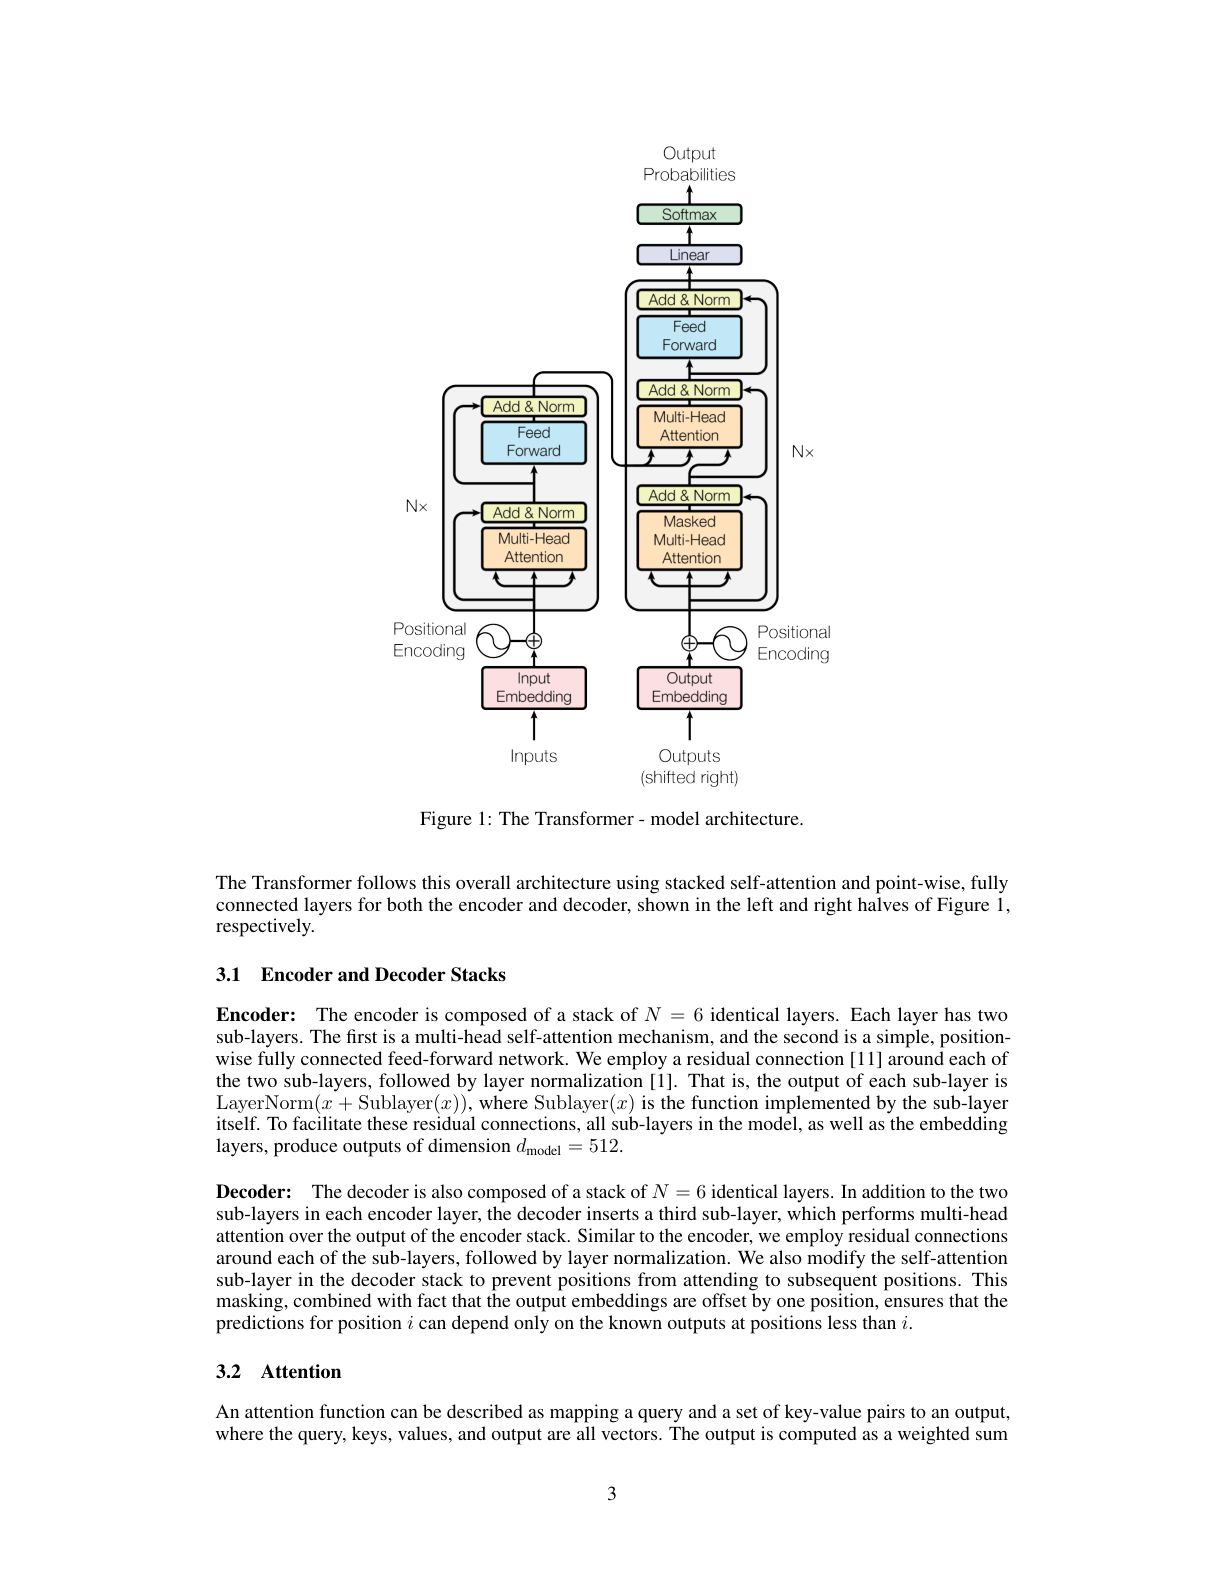
\includegraphics[width=\linewidth,height=0.82\textheight,keepaspectratio]{assets/New-Lecture-Inference_Optimisation/transformer_vaswani_p3.png}\\[-0.2em]
%     {\scriptsize Scaled dot-product attention (Vaswani et al., 2017).}
%   \end{columns}
% \end{frame}

